Let
\begin{align}
\vec{C}\myvec{x\\0}
\end{align}
divide  $\vec{AB} $ in k:1 ratio.
Then, 
\begin{align}
\left(k+1\right)\myvec{x\\0} &=k\myvec{1\\-5} + \myvec{-4\\5}
\\
\implies 0 &= -5k + 5
\\
\text{or, }k&= 1
\\
\vec{C} = \frac{\myvec{-3\\0}}{2} = \myvec{-1.5\\0}
\end{align}
\begin{figure}[!ht]
	\centering
	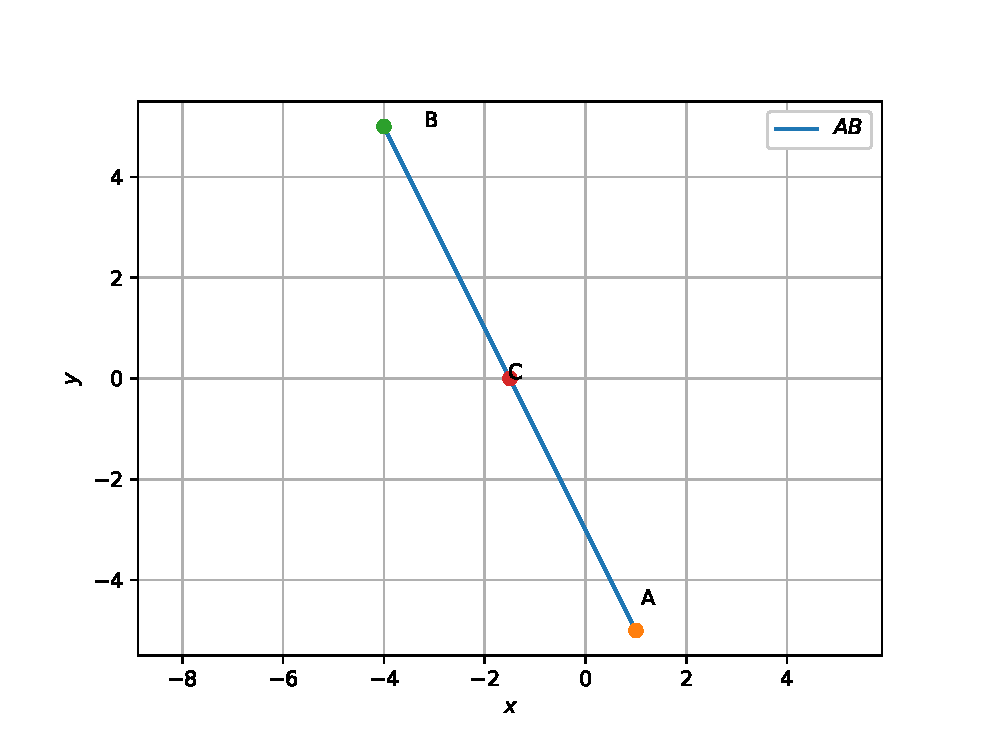
\includegraphics[width=\columnwidth]{./solutions/4/figures/line/point_on_line/point_on_line.eps}
	\caption{line }
	\label{fig:3.6.4_line}
\end{figure}

The following code plots Fig. 	\ref{fig:3.6.4_line}

\begin{lstlisting}
solutions/4/codes/line/point_on_line/points_on_line.py
\end{lstlisting}

